% !TeX program = pdflatex
\documentclass[preprint,12pt]{elsarticle}
\journal{Computer Networks}

\usepackage{amsmath,amssymb,amsfonts}
\usepackage{multirow}
\usepackage{makecell}

\usepackage{textcomp}
\usepackage{xcolor}

\usepackage{algorithm}
\usepackage{algorithmic}
\usepackage{booktabs}
\usepackage{graphicx}
\usepackage{array}
\usepackage{placeins}
\usepackage{tikz}
\usetikzlibrary{arrows.meta,positioning,fit,calc}


\usepackage{amsmath,amssymb,amsfonts}

\usepackage{amsmath,amssymb,amsfonts}
\usepackage{multirow}
\usepackage{makecell}

\usepackage{textcomp}
\usepackage{xcolor}

\usepackage{algorithm}
\usepackage{algorithmic}
\usepackage{booktabs}
\usepackage{graphicx}
\usepackage{array}
\usepackage{tikz}
\usetikzlibrary{arrows.meta,positioning,fit,calc}
\title{Risk-Aware Multicast Scheduling for Federated Learning over Space--Air--Ground Mobile Networks}

% All authors share the three affiliations; + marks the corresponding author.
\author[inst1,inst2,inst3]{Wenyu Ma}
\author[inst1,inst2,inst3]{Tao Hu\corref{cor1}}
\author[inst1,inst2,inst3]{Xinlei Liu}
\cortext[cor1]{Corresponding author}
\ead{hutaondsc@163.com}
\address[inst1]{Information Engineering University, Zhengzhou 450001, China}
\address[inst2]{Key Laboratory of Cyberspace Endogenous Safety and Security of Henan Province, Zhengzhou 450001, China}
\address[inst3]{Key Laboratory of Cyberspace Security, Ministry of Education of China, Zhengzhou 450001, China}

% !TeX program = pdflatex
\begin{document}
\begin{frontmatter}
\begin{abstract}
	Space--air--ground mobile networks turn protected federated learning (FL) into a coupled scheduling problem: mobility affects timely delivery, protection changes deadline feasibility, and operational exposure accumulates across rounds. We formulate mobility-prior risk-budgeted protection selection (MP-RBPS) as a joint client--policy assignment whose estimated action value combines on-time learning contribution, communication and energy costs, update distortion, and residual exposure. Because secure aggregation is a collective operation, we model it as a group-cardinality action with group-size-dependent overhead. We then develop group-cardinality dynamic programming (GCDP), an exact polynomial-time solver for the resulting estimated per-round problem. A five-seed CIFAR-10 evaluation shows that GCDP attains the largest modeled utility in the main experiment and reduces communication relative to reactive and compression-only scheduling, while incurring additional scheduler computation and not maximizing accuracy alone. Controlled stress tests further identify the operating regimes in which fixed, sequential, and low-complexity alternatives remain competitive. MP-RBPS-GCDP therefore contributes a cross-layer decision abstraction and an exact per-round solver, rather than a new cryptographic primitive or a claim of universal accuracy improvement.
\end{abstract}


\begin{keyword}
Federated learning \sep Space--air--ground integrated networks \sep Mobile edge computing \sep Multicast scheduling \sep Privacy-preserving federated learning
\end{keyword}

\end{frontmatter}


\section{Introduction}

Space--air--ground integrated networks support wide-area sensing, emergency response, intelligent transportation, remote monitoring, and edge intelligence by connecting terrestrial devices, UAVs, satellites, edge aggregators, and cloud coordinators \cite{liu2018sagin,mahboob2024ntn,tang2023flsagin}. These networks also create heterogeneous operating conditions: ground clients usually have stable links but limited energy, UAV clients face frequent handovers, and satellite-connected clients suffer long delay, short visibility windows, and outages \cite{mahboob2024ntn,razmi2022ground,qin2024dfrl}.

Federated learning (FL) trains models without uploading raw data \cite{mcmahan2017fedavg,kairouz2021advances}, but model updates can still leak information through reconstruction, inference, or reverse-engineering attacks \cite{zhu2019deep,zhao2025federation}. Differential privacy, secure aggregation, and cryptographic protection reduce such risks \cite{bonawitz2017secureagg,mansouri2023sok,wei2023pfl_dp,yuan2023amplitude}, but they also add computation, communication, synchronization, or accuracy costs \cite{yuan2023privacyresource,zheng2023aggregation}.

This trade-off is sharper in space--air--ground mobile FL. Strong fixed protection can overload low-power clients or cause deadline misses during handovers and satellite outages, whereas lightweight protection may be insufficient for high-risk cross-domain links. Prior work on intermittent clients, satellite FL, and SAGIN-oriented FL shows that mobility, link intermittency, and resource heterogeneity strongly affect participation and convergence \cite{ribero2023intermittent,razmi2022ground,tang2023flsagin,qin2024dfrl}. Thus, client participation and protection-policy selection should be jointly optimized under mobility, deadline, resource, and exposure-budget constraints.

Existing privacy-preserving FL often applies a uniform mechanism across clients or rounds \cite{bonawitz2017secureagg,mansouri2023sok,wei2023pfl_dp}. Communication-efficient wireless FL reduces update size through sparsification, quantization, compressed sensing, over-the-air aggregation, or client selection \cite{oh2023fedqcs,oh2024fedvqcs,liu2023adaptivequant,kim2023beamforming,chen2024clientselection,dong2024aoi}. These two lines of work leave a specific decision gap. A client with a valuable update may be unusable because protection overhead pushes it beyond the round deadline; conversely, repeatedly choosing a timely but weakly protected client can accumulate exposure across rounds. Client admission, protection choice, and inter-round exposure control are therefore coupled decisions rather than independent modules.

This paper develops MP-RBPS-GCDP for deadline-constrained FL over space--air--ground mobile networks. MP-RBPS denotes the cross-layer decision framework, whereas GCDP denotes its exact solver for the estimated per-round assignment. The key abstraction is to make admission and protection a single client--policy action: the same action determines deadline feasibility, resource cost, update distortion, and exposure-budget consumption. Secure aggregation is consequently modeled as a group-cardinality action rather than an always-available per-client switch. This representation exposes a combinatorial structure hidden by sequential admission-then-protection pipelines.

A preliminary poster version introduced the MP-RBPS application setting and used a heuristic admission-and-repair procedure~\cite{ma2026mswim}. The present article substantially reformulates that work: it replaces the heuristic with GCDP and a per-round optimality analysis, models future handover and outage as random events rather than decision-time observations, makes SecAgg overhead group-size dependent, refines the threat and exposure semantics, and reports a new five-seed implementation with exactness checks, additional baselines, calibration diagnostics, and controlled stress scenarios. Accordingly, all numerical conclusions in this article are based on the revised model and implementation and should not be compared directly with the preliminary simulator results.

The main contributions are as follows:
\begin{itemize}
	\item We formulate a joint client--policy selection problem in which the reward is the expected on-time learning contribution, rather than update utility or link reliability alone. The formulation explicitly couples mobility and outage risk with policy-dependent delay, communication, energy, learning degradation, and a cross-round exposure budget.
	
	\item We develop GCDP, an exact group-cardinality solver for the estimated per-round problem. For each feasible SecAgg group size, it compresses each client's policy set into its best non-SecAgg and SecAgg actions and uses dynamic programming to optimize total admission and group membership. We prove conditional per-round optimality and give polynomial complexity in the client and admission caps.
	
	\item We provide an auditable evaluation implementation with common traces, exactness checks against exhaustive enumeration, FedAvg and protection baselines, and explicit reporting of the utility--accuracy--communication--risk trade-off. The implementation separates reliability calibration and downstream learning evaluation and does not interpret the application-level exposure score as formal differential privacy.
\end{itemize}

\subsection{Motivation and contributions}
\label{sec:motivation_contributions}
The practical bottleneck is not the choice of a single cryptographic primitive. It is the interaction between a mobile link and a protected update: a stronger protection mode can increase packet size and processing time, while a handover or visibility interruption can invalidate an otherwise useful participant. Treating admission, multicast protection, and exposure control as sequential decisions therefore hides the network trade-off that determines whether an update reaches the aggregator before the round deadline.

Three limitations in existing networked FL designs motivate our formulation. First, client selection and protection overhead are usually optimized separately, so deadline feasibility is not evaluated for the final protected update. Second, mobile and non-terrestrial FL studies model intermittent connectivity, but rarely carry the resulting uncertainty into a joint multicast decision. Third, secure aggregation is often represented as a per-client switch even though its signaling and recovery cost depends on the participating group. These gaps lead to the following focused contributions:
\begin{itemize}
    \item a network-layer client--policy abstraction that jointly captures mobility-conditioned delivery, deadline feasibility, resource cost, and a bounded exposure state;
    \item an exact group-cardinality dynamic program that returns the optimal assignment for each estimated round and makes its assumptions explicit; and
    \item a trace-driven evaluation with common random numbers, exactness checks, calibration diagnostics, and controlled stress cases that reports both gains and failure regimes.
\end{itemize}
The remainder of this article first reviews related network and FL mechanisms, then defines the architecture and threat model, presents the optimization and solver, and finally evaluates the resulting trade-offs.

\section{Related Work}

\subsection{Privacy-Preserving Federated Learning}

Privacy-preserving FL reduces information exposure during collaborative training \cite{zhao2025federation,kairouz2021advances}. Differential privacy perturbs local updates or aggregated models but introduces a privacy--utility trade-off \cite{wei2023pfl_dp,yuan2023amplitude,yuan2023privacyresource}. Secure aggregation hides individual updates from the server through masking, secret sharing, homomorphic encryption, functional encryption, or secure multi-party computation \cite{bonawitz2017secureagg,mansouri2023sok}. Recent systems further study efficiency, resilience, and deployment issues \cite{zheng2023aggregation}.

The cited studies emphasize privacy guarantees, aggregation security, or the privacy--utility balance \cite{wei2023pfl_dp,yuan2023amplitude,zhao2025federation}. They do not jointly select clients and protection policies under mobility-conditioned delivery, resource, and cross-round exposure constraints.

\subsection{Communication-Efficient Wireless FL}

Communication-efficient FL reduces update overhead through sparsification, pruning, quantization, compressed sensing, over-the-air aggregation, or client selection \cite{oh2023fedqcs,oh2024fedvqcs,liu2023adaptivequant,kim2023beamforming}. Client selection improves efficiency by admitting useful clients under heterogeneous data, latency, and learning capability \cite{oort2021oort,chen2024clientselection,dong2024aoi}. Cost-aware mobile-edge FL also shows that communication, computation, and energy costs should be controlled jointly \cite{luo2021costeffective}.

These methods optimize transmitted bytes, convergence, or latency \cite{oh2023fedqcs,liu2023adaptivequant,chen2024clientselection}, but the cited formulations do not include policy-dependent protection overhead or a cross-round exposure state.

\subsection{FL in Mobile Edge and Non-Terrestrial Networks}

FL has been studied in mobile edge computing, UAV networks, satellite networks, and space--air--ground integrated networks \cite{razmi2022ground,tang2023flsagin,qin2024dfrl}. Ground-assisted FL in LEO constellations highlights visibility windows and asynchronous participation \cite{razmi2022ground}. SAGIN-oriented FL and federated reinforcement learning have also been used for intelligent transmission, offloading, and network optimization \cite{tang2023flsagin,qin2024dfrl}. More broadly, non-terrestrial 6G systems face long delay, handover, spectrum sharing, resource allocation, and intermittent connectivity \cite{mahboob2024ntn,liu2018sagin}.

Recent SAGIN-assisted FL further considers adaptive offloading and seamless handover under satellite coverage dynamics \cite{han2024orchestrating}. These studies establish the importance of mobility, heterogeneous computation, and satellite coverage, but the cited schedulers do not make protection policy part of the admission action.

\subsection{Positioning of This Work}

Table~\ref{tab:related_comparison} positions MP-RBPS at the intersection of protection overhead, mobility-conditioned delivery, client admission, and cross-round exposure control.

\begin{table*}[t]
	\centering
	\caption{Positioning of MP-RBPS against the Closest Research Directions}
	\label{tab:related_comparison}
	\scriptsize
	\setlength{\tabcolsep}{4pt}
	\resizebox{\textwidth}{!}{%
	\begin{tabular}{l c c c c c c}
		\hline
		Research direction & Adaptive client admission & Policy-dependent protection overhead & Mobility/outage information & Round-deadline feasibility & Cross-round exposure state & SecAgg group feasibility \\
		\hline
		Privacy-preserving FL \cite{bonawitz2017secureagg,mansouri2023sok,wei2023pfl_dp} & No & Partial & No & No & DP only & Partial \\
		Communication-efficient wireless FL \cite{oh2023fedqcs,oh2024fedvqcs,liu2023adaptivequant,kim2023beamforming} & Partial & No & No & Partial & No & No \\
		Utility/cost-aware client selection \cite{oort2021oort,chen2024clientselection,dong2024aoi,luo2021costeffective} & Yes & No & Partial & Partial & No & No \\
		Mobile and non-terrestrial FL \cite{razmi2022ground,tang2023flsagin,qin2024dfrl,han2024orchestrating} & Partial & No & Yes & Partial & No & No \\
		MP-RBPS-GCDP & Yes & Yes & Yes & Yes & Yes & Yes \\
		\hline
	\end{tabular}%
	}
\end{table*}

The table summarizes the typical focus of the cited directions; individual systems may support additional features. MP-RBPS-GCDP does not claim novelty for its constituent mechanisms. Its distinct decision unit is the \emph{client--policy pair}, whose feasibility depends on conditional delivery reliability, local resources, remaining exposure budget, and SecAgg group membership.

\section{System and Threat Model}

\subsection{Space-Air-Ground FL Architecture}

We consider a space--air--ground mobile edge network with ground clients, UAV clients or relays, satellite-connected clients, edge aggregators, and a cloud coordinator. The client set is
\begin{equation}
	\mathcal{D} = \mathcal{D}_{g} \cup \mathcal{D}_{a} \cup \mathcal{D}_{s},
\end{equation}
where $\mathcal{D}_{g}$, $\mathcal{D}_{a}$, and $\mathcal{D}_{s}$ denote ground, aerial, and satellite-connected clients, respectively. Ground clients include sensors, smartphones, vehicles, and terrestrial IoT devices. Aerial clients include UAV terminals and UAV-assisted relays. Satellite-connected clients include satellite terminals or remote devices using satellite links.

The edge layer performs regional aggregation, state monitoring, and policy feedback, while the cloud coordinator maintains and aggregates the global FL model. Unlike conventional FL systems with one protection mechanism for all clients, MP-RBPS assigns each admitted client a policy based on its resource state, mobility-link condition, and residual exposure budget.

Fig.~\ref{fig:architecture} illustrates the revised journal architecture. The MP-RBPS module runs at the edge aggregator, where it constructs client--policy actions, evaluates group-size-dependent feasibility, invokes GCDP, and updates the cross-round state only after transmission outcomes are observed.

\begin{figure}[t]
\centering
\resizebox{\columnwidth}{!}{%
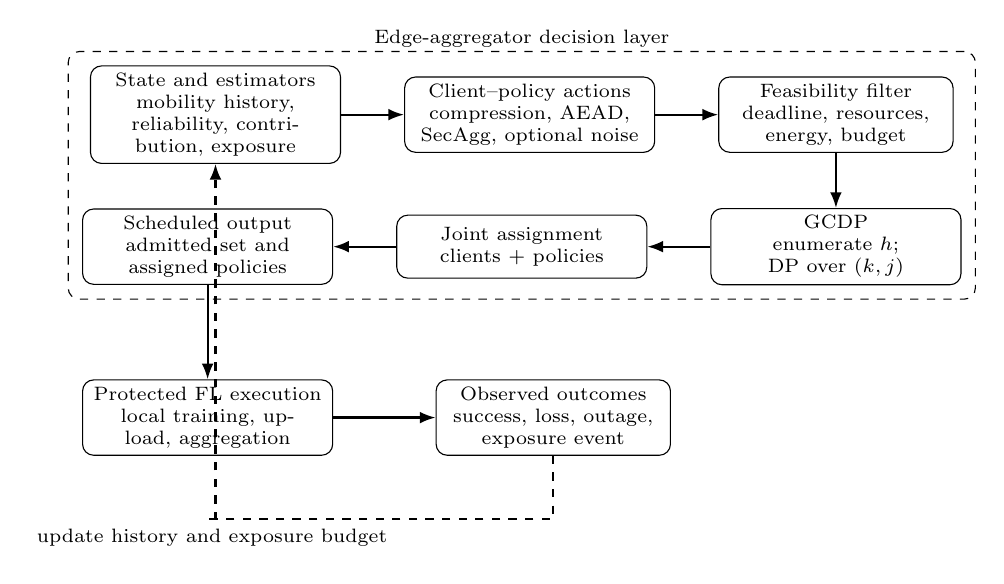
\begin{tikzpicture}[
  node distance=7mm and 8mm, >=Latex,
  box/.style={draw, rounded corners, align=center, minimum height=8mm, text width=30mm, font=\scriptsize, inner sep=2.5pt},
  small/.style={draw, rounded corners, align=center, minimum height=8mm, text width=28mm, font=\scriptsize, inner sep=2.5pt},
  flow/.style={-{Latex[length=2mm]}, thick},
  feedback/.style={-{Latex[length=2mm]}, dashed, thick}
]
\node[box] (estimate) {State and estimators\\mobility history, reliability, contribution, exposure};
\node[box, right=of estimate] (actions) {Client--policy actions\\compression, AEAD, SecAgg, optional noise};
\node[small, right=of actions] (filter) {Feasibility filter\\deadline, resources, energy, budget};
\node[box, below=of filter] (gcdp) {GCDP\\enumerate $h$; DP over $(k,j)$};
\node[box, left=of gcdp] (assign) {Joint assignment\\clients + policies};
\node[box, left=of assign] (output) {Scheduled output\\admitted set and assigned policies};
\node[box, below=12mm of output] (transmit) {Protected FL execution\\local training, upload, aggregation};
\node[small, right=13mm of transmit] (observe) {Observed outcomes\\success, loss, outage, exposure event};
\draw[flow] (estimate) -- (actions);
\draw[flow] (actions) -- (filter);
\draw[flow] (filter) -- (gcdp);
\draw[flow] (gcdp) -- (assign);
\draw[flow] (assign) -- (output);
\draw[flow] (output) -- (transmit);
\draw[flow] (transmit) -- (observe);
\coordinate (feedbacklow) at ($(transmit.south)+(0,-8mm)$);
\draw[feedback] (observe.south) |- (feedbacklow) -| node[below, font=\scriptsize, pos=.28] {update history and exposure budget} (estimate.south);
\node[draw, dashed, rounded corners, fit=(estimate)(actions)(filter)(gcdp)(assign)(output), inner sep=5pt,
      label={[fill=white, inner sep=1pt, font=\scriptsize]above:Edge-aggregator decision layer}] {};
\end{tikzpicture}%
}
\caption{Revised MP-RBPS-GCDP architecture. The edge aggregator jointly selects clients and protection policies with a group-cardinality solver; only observed transmission outcomes update the cross-round state.}
\label{fig:architecture}
\end{figure}

\subsection{FL Workflow}

Each FL round has five steps. First, the cloud broadcasts the global model $w^{t}$ to edge aggregators. Second, each edge aggregator observes the resource and link states of its clients. Third, MP-RBPS constructs feasible client--policy actions and GCDP jointly selects clients, protection classes, and the SecAgg group cardinality. Fourth, selected clients train locally, generate compressed and protected updates, and upload them before deadline $\tau$. Finally, the edge aggregator verifies timely updates, performs regional aggregation, forwards the aggregate to the cloud, and updates the history and exposure budgets from observed outcomes.

Let $\Delta w_i^t$ be the local update of client $i$ in round $t$. An update contributes to aggregation only if it arrives before the deadline and passes integrity verification. Late updates are discarded because stale updates can reduce convergence stability in time-sensitive mobile FL.

\subsection{Mobility, Handover, and Satellite Outage Model}

At the decision instant, each client $i$ exposes an observable state
\begin{equation}
	x_i^t = \left(c_i^t, m_i^t, e_i^t, \bar R_i^t, d_i^t, p_i^t, \boldsymbol{\zeta}_i^t\right),
\end{equation}
where $c_i^t$, $m_i^t$, $e_i^t$, $\bar R_i^t$, $d_i^t$, and $p_i^t$ denote CPU capacity, memory, residual energy, estimated uplink rate, delay, and packet-loss probability, respectively. The vector $\boldsymbol{\zeta}_i^t$ contains available mobility features, such as location, serving-node identity, velocity, and link trend. The actual handover event $H_i^t\in\{0,1\}$ is not known before selection; it is a random event conditioned on the observable state and history. This separation prevents future handover information from leaking into the decision.

For policy $q$, the update delivery time is
\begin{equation}
	T_i^t(q) =
	T_{\mathrm{train},i}^t
	+ T_{\mathrm{proc},i}^t(q)
	+ \frac{B_i^t(q)}{R_i^t}
	+ d_i^t
	+ H_i^t \Delta d_h,
	\label{eq:delivery_time}
\end{equation}
where $T_{\mathrm{train},i}^t$ is local training time, $T_{\mathrm{proc},i}^t(q)$ is compression/protection processing time, $B_i^t(q)$ is protected update size, $R_i^t$ is the realized uplink rate around the estimate $\bar R_i^t$, and $\Delta d_h$ is handover delay. Thus, $T_i^t(q)$ is random before transmission because $R_i^t$ and $H_i^t$ are not yet realized.

Handover also increases packet loss:
\begin{equation}
	\tilde{p}_i^t(H_i^t) = \min \left(1, p_i^t + H_i^t \Delta p_h \right),
	\label{eq:handover_loss}
\end{equation}
where $\Delta p_h$ is the handover loss penalty. Let $J_i^t\in\{0,1\}$ indicate packet loss and use $\Pr(J_i^t=1\mid H_i^t,x_i^t)=\tilde p_i^t(H_i^t)$. Satellite-connected clients may also suffer a random visibility-window interruption $O_i^t\in\{0,1\}$; for terrestrial clients, $O_i^t=0$. An update succeeds only if it arrives before the deadline and neither loss nor outage occurs.

\subsection{Threat and Protection Model}
\label{sec:threat}

We consider three threat surfaces in space--air--ground FL: external eavesdropping on wireless links, tampering or replay during cross-domain relaying, and an honest-but-curious edge aggregator that may infer information from individual updates.

MP-RBPS uses standard protection mechanisms rather than new cryptographic primitives. AEAD schemes such as AES-GCM and ChaCha20-Poly1305 protect update confidentiality and integrity over wireless and cross-domain links~\cite{nist2007gcm,rfc8439}. In deployment, associated data should include round identifiers, client identifiers, and sequence numbers, and nonce uniqueness must be enforced. AEAD protects transmitted updates but does not hide decrypted individual updates from an authorized aggregator. Secure aggregation therefore limits aggregator-side exposure by revealing only group aggregates. Differential privacy can be enabled for high-risk policies by adding calibrated noise to clipped updates, at the cost of utility loss~\cite{wei2023pfl_dp,yuan2023amplitude,yuan2023privacyresource}.

Section~\ref{sec:exposure_budget} defines a threat-specific exposure score for scheduling; formal differential-privacy accounting remains separate.

\section{Risk-Budgeted Protection Selection Problem}

\subsection{Candidate Protection Policies}

At each FL round, the edge aggregator selects a policy from candidate set $\mathcal{Q}$. A policy specifies pruning ratio, quantization level, transmission protection, secure aggregation, and optional differential privacy:
\begin{equation}
	q_i^t = \left(\rho_i^t, z_i^t, a_i^t, g_i^t, \sigma_i^t\right),
	\label{eq:policy_tuple}
\end{equation}
where $\rho_i^t$ is the pruning ratio, $z_i^t$ is the quantization bit-width, $a_i^t$ is the transmission protection mode, $g_i^t\in\{0,1\}$ indicates secure aggregation, and $\sigma_i^t$ is the Gaussian-noise multiplier after clipping. When DP is disabled, $\sigma_i^t=0$. The multiplier is not itself a privacy parameter; a formal $(\epsilon,\delta)$ value must be computed from the sampling rate, number of compositions, clipping rule, and an explicit DP accountant.

Table~\ref{tab:policy_set} shows the candidate policies. Compression reduces update size, authenticated encryption with associated data (AEAD) protects transmission, secure aggregation (SecAgg) limits aggregator-side visibility, and Gaussian noise can support differential privacy when accompanied by a valid accountant. Let $k_{\mathrm{SA}}^t$ denote the number of admitted clients assigned a SecAgg policy. For $g_i^t=1$, processing time, communication cost, energy, and delivery reliability may depend on $k_{\mathrm{SA}}^t$ because group setup and dropout recovery are collective operations. We suppress this argument in general equations and restore it in the solver below.

\begin{table}[t]
	\centering
	\caption{Candidate Protection Policy Set}
	\label{tab:policy_set}
	\scriptsize
	\setlength{\tabcolsep}{3pt}
	\begin{tabular}{c c c c c c}
		\hline
		Policy & Pruning & Quant. & AEAD & SecAgg & Noise \\
		\hline
		$q_1$ & 0\%  & 32-bit & Yes & No  & No \\
		$q_2$ & 30\% & 16-bit & Yes & No  & No \\
		$q_3$ & 50\% & 8-bit  & Yes & No  & No \\
		$q_4$ & 50\% & 8-bit  & Yes & Yes & No \\
		$q_5$ & 70\% & 8-bit  & Yes & Yes & Yes \\
		\hline
	\end{tabular}
\end{table}

\subsection{Useful Update Contribution}

Stable connectivity does not always imply high learning value. We define a lightweight useful contribution score:
\begin{equation}
	G_i^t =
	\omega_1
	\frac{n_i}{\sum_{j \in \mathcal{D}} n_j}
	+
	\omega_2
	\frac{\kappa^{t-\ell(i,t)}\|\Delta w_i^{\ell(i,t)}\|_2}
	{\sum_{j \in \mathcal{D}}\kappa^{t-\ell(j,t)}\|\Delta w_j^{\ell(j,t)}\|_2 + \xi}
	+
	\omega_3 D_i
	+
	\omega_4 F_i,
	\label{eq:contribution}
\end{equation}
where $n_i$ is local data size, $\|\Delta w_i^{\ell(i,t)}\|_2$ is the norm from client $i$'s most recent successful participation $\ell(i,t)<t$, $D_i\in[0,1]$ is a data-diversity proxy, $F_i\in[0,1]$ is a domain-fairness weight, and $\xi>0$ avoids division by zero. The weights satisfy $\omega_k\geq0$ and $\sum_{k=1}^4\omega_k=1$. For a client with no previous update, we set $\ell(i,t)=0$ and replace its norm by the median initial norm in the same domain. Stale norms are multiplied by a recency factor $\kappa^{t-\ell(i,t)}$, $0<\kappa\leq1$. If labels are not server-visible, $D_i$ must be obtained from an explicitly specified privacy-preserving summary; otherwise that term is disabled. Because a large update norm may also indicate noise or abnormal behavior, $G_i^t$ is a scheduling heuristic rather than an exact marginal loss reduction.

\subsection{Deadline-Aware Timely-Update Reliability}

Each edge aggregator maintains a historical failure prior from recent bandwidth, delay, packet loss, handover, and outage observations $\mathcal{H}_i^{t-L:t-1}$:
\begin{equation}
	\hat{r}_i^t = f_{\phi}\left(\mathcal{H}_i^{t-L:t-1}, x_i^t\right),
\end{equation}
where $f_{\phi}(\cdot)$ can be an EWMA, logistic model, or small neural predictor. The default lightweight estimator is
\begin{equation}
	\hat{r}_i^t =
	\begin{cases}
	\lambda \hat{r}_i^{t-1}+(1-\lambda)r_i^{t-1},
	& \text{if an outcome was observed at }t-1,\\
	\hat{r}_i^{t-1}, & \text{otherwise},
	\end{cases}
	\label{eq:ewma}
\end{equation}
where $r_i^{t-1}=1$ if client $i$ experienced timeout, packet loss, handover failure, or satellite outage in round $t-1$, and $0$ otherwise. A nonparticipating client provides no new outcome, so its prior is carried forward rather than updated repeatedly from stale data. We initialize $\hat r_i^0$ with the empirical failure rate of the corresponding ground, aerial, or satellite-connected domain. EWMA is a history-aware estimator rather than a trajectory predictor.

Define the successful-delivery event
\begin{equation}
	Y_i^t(q)=\mathbf{1}\!\left\{T_i^t(q)\leq\tau,\;J_i^t=0,\;O_i^t=0\right\}.
	\label{eq:success_event}
\end{equation}
For policy $q$, timely-update reliability is the joint conditional probability
\begin{equation}
	P_{\mathrm{rel},i}^{t}(q)
	=
	\Pr\!\left(Y_i^t(q)=1\mid \mathcal{H}_i^{t-L:t-1},x_i^t,q\right).
	\label{eq:reliability_score}
\end{equation}

This joint definition does not multiply overlapping timeout, loss, outage, and historical-failure terms and therefore does not require an independence assumption among them. It can be estimated by sampling a stated conditional link model or learned and calibrated from binary outcomes $Y_i^t$. The value $\hat r_i^t$ is a deterministic summary of the conditioning history and may be supplied to the estimator as a feature; it is not an additional multiplicative probability factor. Calibration should be assessed using a proper score such as the Brier score or expected calibration error.

\subsection{Residual Exposure Budget}
\label{sec:exposure_budget}

Each client maintains a residual exposure budget $\Gamma_i^t$. The exposure cost of policy $q$ is $R_{\mathrm{exp}}(q)$, where a smaller value indicates lower measured exposure under Section~\ref{sec:threat}. This application-level score is not a DP loss, attack success probability, or cryptographic security level.

\begin{table}[t]
	\centering
	\caption{Threat-Specific Exposure-Cost Classes}
	\label{tab:risk_cost}
	\scriptsize
	\setlength{\tabcolsep}{3pt}
	\renewcommand{\arraystretch}{1.12}
	\begin{tabular}{c >{\raggedright\arraybackslash}p{0.58\columnwidth} c}
		\hline
		Policy & Protection mode & $R_{\mathrm{exp}}(q)$ \\
		\hline
		$q_1$ & AEAD only & $r_{\mathrm{A}}$ \\
		$q_2$ & Pruning + 16-bit quantization + AEAD & $r_{\mathrm{A}}$ \\
		$q_3$ & Pruning + 8-bit quantization + AEAD & $r_{\mathrm{A}}$ \\
		$q_4$ & $q_3$ + SecAgg & $r_{\mathrm{S}}$ \\
		$q_5$ & $q_4$ + Gaussian noise & $r_{\mathrm{D}}$ \\
		\hline
	\end{tabular}
\end{table}



The costs satisfy $0\leq r_{\mathrm{D}}\leq r_{\mathrm{S}}<r_{\mathrm{A}}$ only after calibration for the stated threat. Policies $q_1$--$q_3$ receive the same cost because compression alone does not provide a formal privacy guarantee. A defensible calibration can use reconstruction error, membership-inference advantage, or another threat-specific empirical measure on held-out data. The value $r_{\mathrm{D}}$ is an application-level exposure score; formal differential-privacy loss must be maintained separately by a standard accountant.


Let $\chi_i^t\in\{0,1\}$ indicate that client $i$ transmitted an update far enough for the threat-specific exposure event to occur; hence $\chi_i^t\leq s_i^t$. Before selection, its conditional probability under policy $q$ is
\begin{equation}
	\pi_{\mathrm{exp},i}^t(q)=
	\Pr\!\left(\chi_i^t=1\mid \mathcal H_i^{t-L:t-1},x_i^t,q,s_i^t=1\right).
	\label{eq:exposure_probability}
\end{equation}
Budgets are updated after each round by
\begin{equation}
	\Gamma_i^{t+1}
	=
	\max\left(0,\Gamma_i^t - \chi_i^t R_{\mathrm{exp}}(q_i^t)\right).
	\label{eq:budget_update}
\end{equation}
Thus, non-participating clients do not consume budget, whereas repeated exposed transmissions under high-cost policies exhaust it faster. The exact definition of $\chi_i^t$ must follow the threat model: for link eavesdropping it becomes one when transmission starts, while for aggregator-side exposure it becomes one only when an individually visible update reaches the aggregator. We treat the budget as a finite-horizon control variable for one FL task; long-running deployments can use sliding-window budgets or task-level resets.

\subsection{Optimization Objective}

At round $t$, the edge aggregator jointly decides admission $s_i^t\in\{0,1\}$ and policy $q_i^t$. The objective maximizes expected useful contribution while penalizing communication cost, energy cost, predicted update distortion, and expected measured exposure:
\begin{equation}
	\begin{aligned}
		\max_{\{s_i^t,q_i^t\}}
		\sum_{i \in \mathcal{D}}
		s_i^t
		\Big[
		&G_i^t P_{\mathrm{rel},i}^{t}(q_i^t)
		- \alpha \hat{B}_i^t(q_i^t)
		- \beta \hat{E}_i^t(q_i^t)  \\
		&- \gamma \hat{A}_{\mathrm{loss},i}^t(q_i^t)
		- \delta \pi_{\mathrm{exp},i}^t(q_i^t)R_{\mathrm{exp}}(q_i^t)
		\Big],
	\end{aligned}
	\label{eq:objective}
\end{equation}
subject to
\begin{equation}
	s_i^t=1\;\Longrightarrow\;P_{\mathrm{rel},i}^{t}(q_i^t) \geq \theta,
	\label{eq:reliability_constraint}
\end{equation}
\begin{equation}
	s_i^t=1\;\Longrightarrow\;C_i^t(q_i^t) \leq c_i^t,
	\label{eq:cpu_constraint}
\end{equation}
\begin{equation}
	s_i^t=1\;\Longrightarrow\;M_i^t(q_i^t) \leq m_i^t,
	\label{eq:memory_constraint}
\end{equation}
\begin{equation}
	s_i^t=1\;\Longrightarrow\;E_i^t(q_i^t) \leq e_i^t,
	\label{eq:energy_constraint}
\end{equation}
\begin{equation}
	s_i^t=1\;\Longrightarrow\;R_{\mathrm{exp}}(q_i^t) \leq \Gamma_i^t,
	\label{eq:risk_constraint}
\end{equation}
\begin{equation}
	\sum_{i \in \mathcal{D}} s_i^t \leq K,
	\label{eq:admission_constraint}
\end{equation}
\begin{equation}
	k_{\mathrm{SA}}^t=
	\sum_{i \in \mathcal{D}} s_i^t \mathbf{1}\{g_i^t=1\},
	\qquad
	k_{\mathrm{SA}}^t\in\{0\}\cup\{m_{\min},\ldots,K\}.
	\label{eq:secagg_group_constraint}
\end{equation}
The bracketed term in (\ref{eq:objective}) is denoted by $U_i^t(q)$. The weights $\alpha$, $\beta$, $\gamma$, and $\delta$ are nonnegative and control communication, energy, distortion, and expected-exposure penalties, respectively. The objective uses $\pi_{\mathrm{exp},i}^t(q)R_{\mathrm{exp}}(q)$, whereas constraint (\ref{eq:risk_constraint}) reserves enough budget for the worst-case exposure event. Here, $\theta$ is the reliability target, $K$ is the admission budget, and $m_{\min}$ is the minimum secure-aggregation group size. The implication form ensures that per-client feasibility is required only for admitted clients. The quantities $C_i^t(q)$ and $M_i^t(q)$ are the predicted CPU and memory demands, checked against the observed capacities $c_i^t$ and $m_i^t$. Actual energy $E_i^t(q)$ is checked against residual energy $e_i^t$, whereas $\hat E_i^t(q)$ is a dimensionless objective term. We use bounded normalizations $\hat B_i^t(q)=B_i^t(q)/B_{\max}$ and $\hat E_i^t(q)=E_i^t(q)/E_{\max}$, with constants fixed across all compared methods. Let the realized relative update distortion be
\begin{equation}
	A_{\mathrm{dist},i}^t(q)=
	\min\!\left\{1,
	\frac{\|\Delta w_i^t-\mathcal{C}_q(\Delta w_i^t)\|_2}
	{\|\Delta w_i^t\|_2+\xi}\right\},
	\label{eq:update_distortion}
\end{equation}
where $\mathcal C_q$ is the compression-and-perturbation operator. Because admission occurs before the current update is available, the objective uses the conditional prediction $\hat A_{\mathrm{loss},i}^t(q)=\mathbb E[A_{\mathrm{dist},i}^t(q)\mid\mathcal H_i^{t-L:t-1},x_i^t,q]$. The implementation records this simulator-defined prediction separately from realized downstream accuracy. The group-size constraint prevents secure aggregation from being assigned to too few clients, but it remains a first-order abstraction of a full dropout-resilient SecAgg protocol.

\subsection{Group-Cardinality Decomposition}

For a candidate SecAgg group size \(h\in\mathcal K_{\mathrm{SA}}\), where
\begin{equation}
	\mathcal K_{\mathrm{SA}}=\{0\}\cup\{m_{\min},\ldots,K\},
\end{equation}
all group-dependent quantities can be evaluated conditionally on \(k_{\mathrm{SA}}^t=h\). Let \(\mathcal F_{i,\mathrm N}^t\) be the feasible non-SecAgg policies of client \(i\), and let \(\mathcal F_{i,\mathrm S}^t(h)\) be its feasible SecAgg policies at group size \(h\). Define
\begin{equation}
	N_i^t=\max_{q\in\mathcal F_{i,\mathrm N}^t}U_i^t(q),
	\qquad
	S_i^t(h)=\max_{q\in\mathcal F_{i,\mathrm S}^t(h)}U_i^t(q;h),
	\label{eq:compressed_actions}
\end{equation}
with value \(-\infty\) when the corresponding set is empty. The maximizing policies are stored for reconstruction. This compression is lossless because an admitted client assigned a given protection class never benefits from a lower-utility feasible policy in that class.

For fixed \(h\), let \(V_i^{(h)}(k,j)\) be the maximum utility obtainable from the first \(i\) clients after admitting \(k\) clients in total, exactly \(j\) of whom use SecAgg. Initialize \(V_0^{(h)}(0,0)=0\) and all other states to \(-\infty\). The recurrence is
\begin{equation}
\begin{aligned}
V_i^{(h)}(k,j)=\max\big\{&
V_{i-1}^{(h)}(k,j),\\
&V_{i-1}^{(h)}(k-1,j)+N_i^t,\\
&V_{i-1}^{(h)}(k-1,j-1)+S_i^t(h)
\big\},
\end{aligned}
\label{eq:gcdp_recurrence}
\end{equation}
where invalid indices and infeasible actions have value \(-\infty\). The first, second, and third transitions skip client \(i\), admit it with a non-SecAgg policy, and admit it with a SecAgg policy, respectively. The best value for target \(h\) is
\begin{equation}
	W^t(h)=\max_{h\leq k\leq K}V_{|\mathcal D|}^{(h)}(k,h).
	\label{eq:gcdp_target}
\end{equation}
GCDP selects \(h^*\in\arg\max_{h\in\mathcal K_{\mathrm{SA}}}W^t(h)\) and reconstructs the client--policy assignment from backpointers.

\paragraph{Per-round optimality}
For every fixed \(h\), recurrence (\ref{eq:gcdp_recurrence}) considers all mutually exclusive actions for client \(i\) and retains the best value for each pair \((k,j)\). Induction on \(i\) therefore establishes that \(V_i^{(h)}(k,j)\) is optimal for its state. Equation (\ref{eq:gcdp_target}) covers every feasible admission count for that target, and enumeration of \(\mathcal K_{\mathrm{SA}}\) covers every group cardinality allowed by (\ref{eq:secagg_group_constraint}). Hence GCDP returns a globally optimal solution of the stated per-round problem, conditional on the estimated utilities and group-size-dependent costs.

\section{GCDP-Based MP-RBPS Algorithm}

MP-RBPS first estimates client state, conditional delivery reliability, expected exposure, and update distortion. It then filters policies using the per-client constraints and evaluates the compressed actions in (\ref{eq:compressed_actions}). GCDP replaces greedy admission and post-hoc group repair: SecAgg membership, total admission, and policy class are selected jointly.

Evaluating all client--policy pairs for all candidate group sizes costs \(O(|\mathcal D||\mathcal Q|K)\). For a fixed \(h\), the dynamic program has \(O(Kh)\) states per client; summing over all \(h\leq K\) gives time complexity \(O(|\mathcal D|K^3)\). Rolling arrays require \(O(K^2)\) value memory, while backpointer reconstruction requires \(O(|\mathcal D|K^2)\) memory or a second pass. When SecAgg utility is independent of group size, a single two-count dynamic program reduces the time to \(O(|\mathcal D|K^2)\).

\begin{algorithm}[t]
	\caption{MP-RBPS with Group-Cardinality Dynamic Programming}
	\label{alg:mprbps}
	\begin{algorithmic}[1]
		\REQUIRE Clients \(\mathcal D\), policies \(\mathcal Q\), admission cap \(K\), minimum SecAgg size \(m_{\min}\), states and histories, budgets \(\{\Gamma_i^t\}\)
		\ENSURE Admitted set \(\mathcal S^t\) and assigned policies
		\STATE Estimate \(G_i^t\), \(\hat r_i^t\), and policy-dependent quantities for all clients
		\STATE \(\mathcal K_{\mathrm{SA}}\leftarrow\{0\}\cup\{m_{\min},\ldots,K\}\)
		\FOR{each \(h\in\mathcal K_{\mathrm{SA}}\)}
			\STATE Compute \(N_i^t\), \(S_i^t(h)\), and their maximizing policies for every \(i\)
			\STATE Initialize \(V_0^{(h)}(0,0)=0\); set other states to \(-\infty\)
			\FOR{each client \(i\in\mathcal D\)}
				\FOR{\(0\leq k\leq K\) and \(0\leq j\leq\min(h,k)\)}
					\STATE Apply skip, non-SecAgg, and SecAgg transitions in (\ref{eq:gcdp_recurrence})
					\STATE Store the maximizing transition as a backpointer
				\ENDFOR
			\ENDFOR
			\STATE \(W^t(h)\leftarrow\max_{h\leq k\leq K}V_{|\mathcal D|}^{(h)}(k,h)\)
		\ENDFOR
		\STATE \(h^*\leftarrow\arg\max_{h\in\mathcal K_{\mathrm{SA}}}W^t(h)\)
		\STATE Backtrack to recover \(\mathcal S^t\) and the client--policy assignment
		\STATE After transmission, observe \(\chi_i^t\) and update \(\Gamma_i^{t+1}\) by (\ref{eq:budget_update})
		\RETURN \(\mathcal S^t\) and assigned policies
	\end{algorithmic}
\end{algorithm}

\section{Evaluation Protocol}
\label{sec:evaluation_protocol}

A rigorous evaluation of MP-RBPS-GCDP couples learning dynamics with time-correlated link events while keeping reliability estimation, scheduling utility, and security measurement distinct. We use this protocol for the main CIFAR-10 experiment and a complementary controlled stress study.

\subsection{Experimental Design}

The evaluation uses non-IID CIFAR-10 as a controlled learning task and a space--air--ground client population containing terrestrial, UAV, and satellite-connected clients. Link realizations are generated as time-correlated traces of rate, delay, packet loss, handover, and satellite visibility rather than independent per-round draws. Every compared method receives the same client data partitions, model initialization, and common-random-number traces. The main experiment reports five independent seeds with means and standard deviations.

For each candidate policy, the estimator in (\ref{eq:reliability_score}) is evaluated separately from downstream learning using the Brier score and expected calibration error (ECE), in addition to the observed timeout rate. The EWMA term is treated as a history-aware prior rather than as a trajectory forecast.

The implementation records update size, processing latency, and normalized energy for every selected action and makes SecAgg processing a function of group size. Because no external reconstruction or membership-inference experiment is used to calibrate Table~\ref{tab:risk_cost}, policies that differ only in compression share the same exposure cost. The reported energy and exposure quantities are therefore simulator-normalized costs, not device measurements or attack probabilities.

\subsection{Baselines and Fair Comparison}

The comparison includes FedAvg~\cite{mcmahan2017communication}, fixed AEAD, fixed SecAgg~\cite{bonawitz2017secureagg}, compression-only, a current-state reactive scheduler, a two-stage scheduler that selects clients before assigning protection policies, and greedy repair. The two-stage and greedy baselines isolate the joint action-space and exact-solver contributions, respectively.

All adaptive methods use the same candidate set, admission cap, deadline, training budget, and realized traces. Secure-aggregation baselines share the same minimum group constraint and group-dependent cost model. The Gaussian-noise policy is not labelled as differentially private because the study does not report a sampling rule, \(\delta\), or cumulative \(\epsilon\) from a formal accountant.

\subsection{Metrics and Controlled Stress Study}

The primary learning metric is test accuracy versus communication round. Network metrics are timely-update ratio, transmitted bytes, and normalized energy; scheduling metrics include modeled objective, remaining exposure budget, and solver time. Brier score and ECE characterize delivery-reliability estimates but do not measure privacy.

In addition to the main CIFAR-10 experiment, a lightweight NumPy FL task is used to isolate scheduler behavior across seven controlled settings: nominal operation, high mobility, a tighter deadline, low and high initial exposure budgets, a larger SecAgg minimum group, and a higher exposure penalty. Each setting uses five paired seeds and common random traces. Across the resulting 35 paired runs, GCDP has a higher modeled objective than fixed SecAgg by $0.0992$ (95\% descriptive CI $[0.0663,0.1320]$), compression-only by $1.4258$ ($[1.2152,1.6364]$), and fixed AEAD by $2.6975$ ($[2.4890,2.9059]$). Relative to the sequential two-stage policy, the difference is $-0.1889$ ($[-0.2301,-0.1476]$): GCDP instead provides slightly higher accuracy and lower communication and normalized energy in this controlled matrix. Its objective difference from greedy repair and reactive scheduling is inconclusive. GCDP reduces communication relative to compression-only and fixed SecAgg by approximately $4.8$ normalized units, while adding approximately $57.7$ ms of solver time in this implementation. The stress study therefore identifies a conditional Pareto trade-off rather than universal dominance; it is not pooled with the CIFAR-10 table below.

\subsection{Completed CIFAR-10 results}
The completed five-seed experiment used 500 clients, 150 rounds, an admission cap of 25, and a minimum SecAgg group of 5. Table~\ref{tab:completed_results} reports mean $\pm$ standard deviation across seeds. These values are generated by the accompanying reproducibility project.

\begin{table}[t]
\centering
\caption{Completed CIFAR-10 results (five seeds). ``Objective'' is the modeled per-round utility, not test accuracy.}
\label{tab:completed_results}
\resizebox{\columnwidth}{!}{%
\begin{tabular}{lccccc}
\toprule
Method & Accuracy & Objective & Solver (ms) & Bytes & Budget\\
\midrule
GCDP & $0.5681\!\pm\!0.0108$ & $4.1004\!\pm\!0.0466$ & 1258.5 & 423.97 & 17.12\\
Greedy repair & $0.5695\!\pm\!0.0084$ & $4.0571\!\pm\!0.0391$ & 23.2 & 425.06 & 17.12\\
Two-stage & $0.5536\!\pm\!0.0084$ & $3.6167\!\pm\!0.1202$ & 51.4 & 355.03 & 17.93\\
Reactive & $0.5991\!\pm\!0.0070$ & $2.9220\!\pm\!0.0458$ & 0.6 & 479.06 & 12.50\\
Fixed SecAgg & $0.5667\!\pm\!0.0132$ & $3.6312\!\pm\!0.0411$ & 7.5 & 421.33 & 18.28\\
Compression-only & $0.5986\!\pm\!0.0094$ & $2.9091\!\pm\!0.0508$ & 0.5 & 468.75 & 12.50\\
Fixed AEAD & $0.5815\!\pm\!0.0108$ & $-2.0584\!\pm\!0.0317$ & 0.4 & 3750.00 & 12.50\\
FedAvg & $0.5783\!\pm\!0.0143$ & $-2.0098\!\pm\!0.0316$ & 0.4 & 3750.00 & 12.50\\
\bottomrule
\end{tabular}
}
\end{table}

GCDP obtains the largest modeled utility and reduces transmitted bytes relative to reactive and compression-only scheduling, while requiring substantially more scheduling computation. Its lower test accuracy than reactive and compression-only is not contradictory: the optimized utility also penalizes exposure, energy, distortion, and deadline risk. Thus the experiment supports joint risk--resource optimization rather than universal accuracy superiority. The exposure score remains an application-level quantity; no formal privacy claim is made without a threat-specific attack calibration.

Figure~\ref{fig:completed_accuracy} visualizes the learning trajectories across the five seeds. The reactive and compression-only policies reach higher accuracy because they spend less modeled utility on protection and exposure control; GCDP instead trades a small amount of downstream accuracy for a higher cross-layer objective. Figure~\ref{fig:completed_overheads} reports the corresponding solver/delivery overhead and selected-policy distribution.

\begin{figure}[!t]
\centering
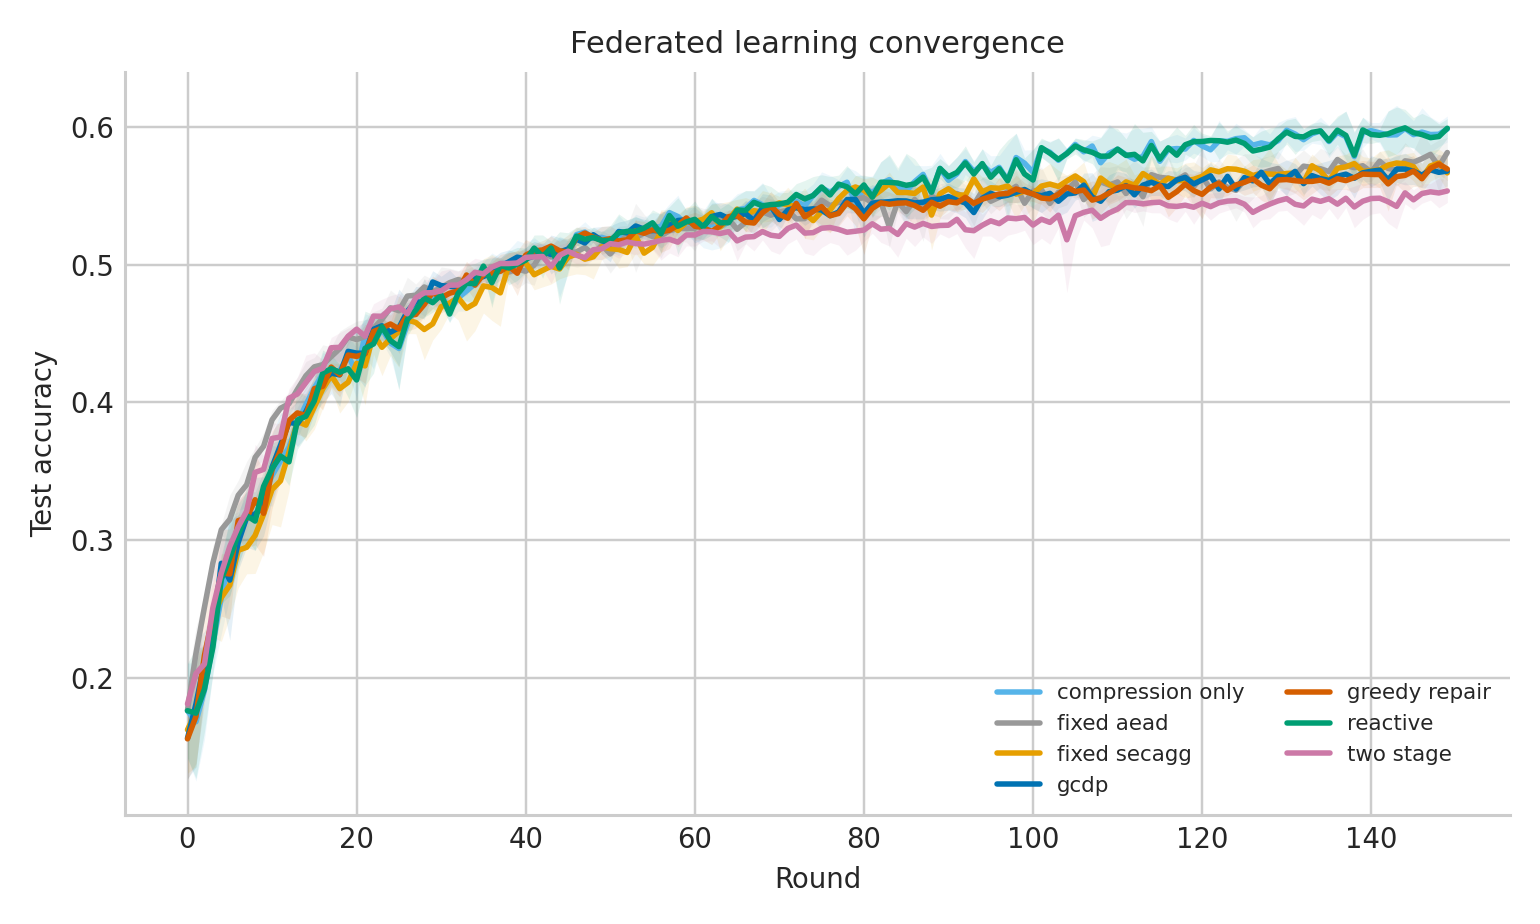
\includegraphics[width=0.98\columnwidth]{accuracy_pub.png}
\caption{CIFAR-10 test accuracy over communication rounds for the completed five-seed experiment. Shaded regions show the across-seed standard deviation.}
\label{fig:completed_accuracy}
\end{figure}

\begin{figure}[!t]
\centering
\begin{minipage}{0.49\columnwidth}
\centering
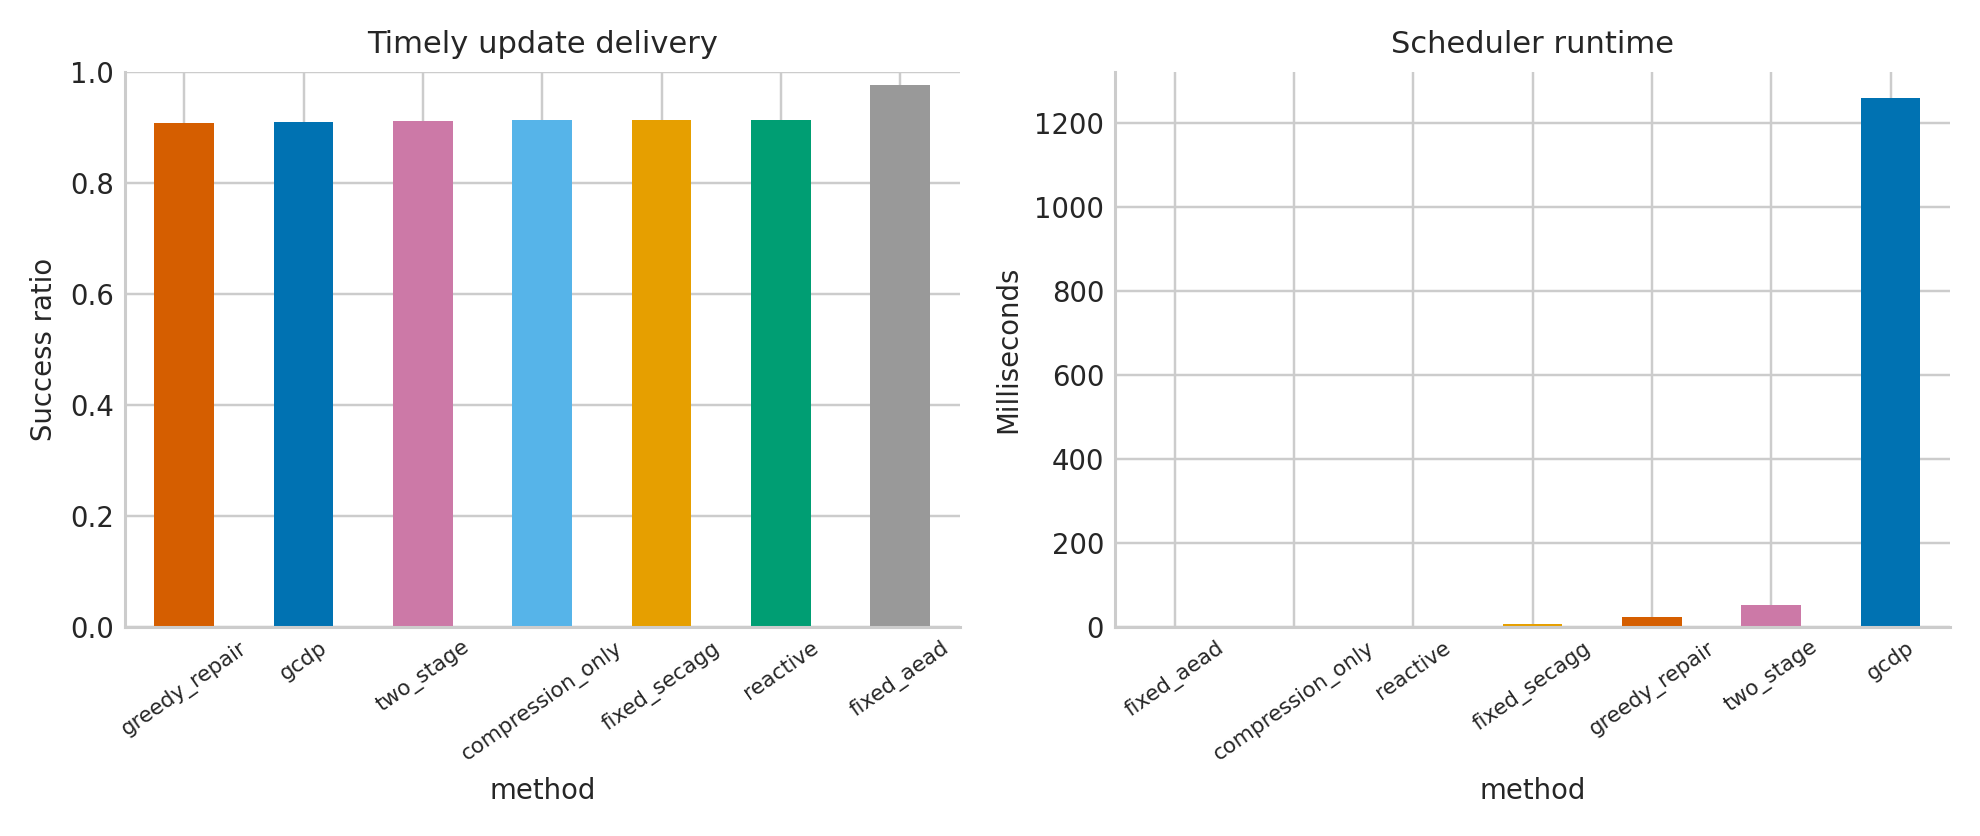
\includegraphics[width=\textwidth]{delivery_runtime_pub.png}
\\[-2pt]\textbf{(a)} Timely delivery and scheduler runtime
\end{minipage}\hfill
\begin{minipage}{0.49\columnwidth}
\centering
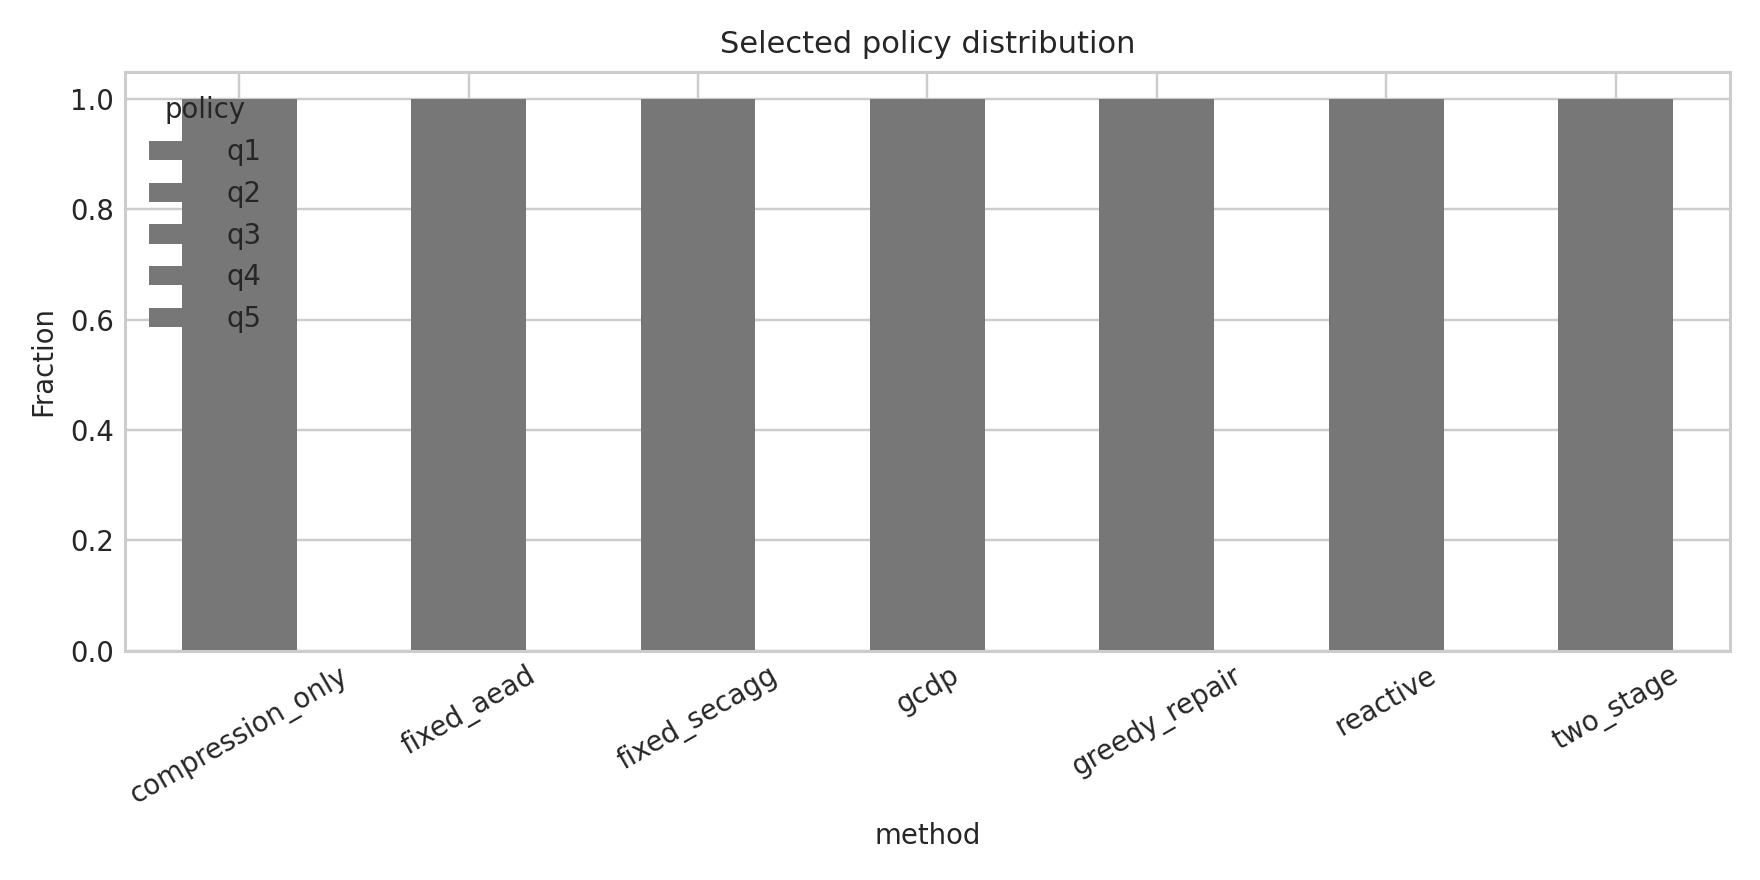
\includegraphics[width=\textwidth]{policy_distribution_pub.png}
\\[-2pt]\textbf{(b)} Selected policy distribution
\end{minipage}
\caption{Completed-experiment overhead and policy usage. Left: delivery success/runtime summary; right: distribution of selected protection policies.}
\label{fig:completed_overheads}
\end{figure}

\begin{figure}[!t]
\centering
\begin{minipage}{0.58\columnwidth}
\centering
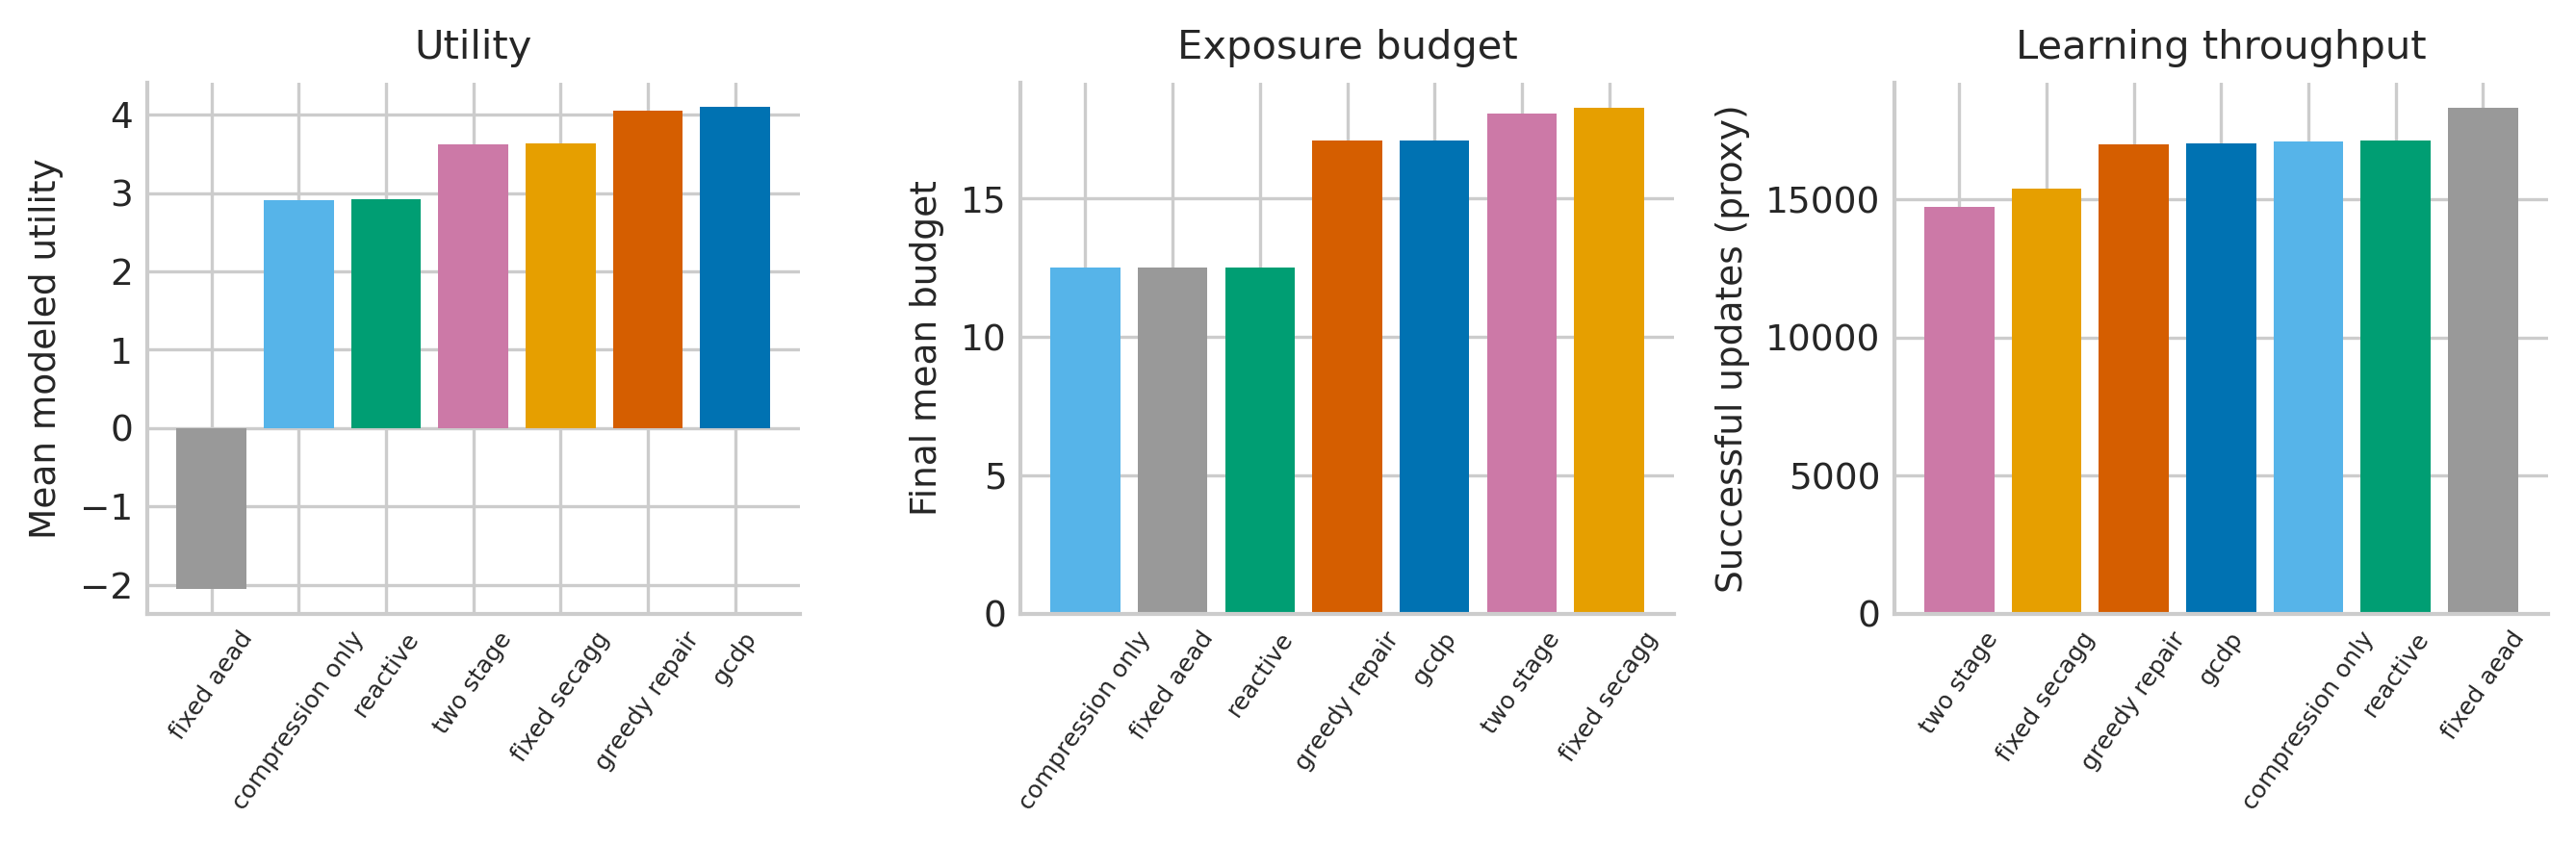
\includegraphics[width=\textwidth]{utility_budget_throughput.png}
\\[-2pt]\textbf{(a)} Utility, budget, and throughput
\end{minipage}\hfill
\begin{minipage}{0.38\columnwidth}
\centering
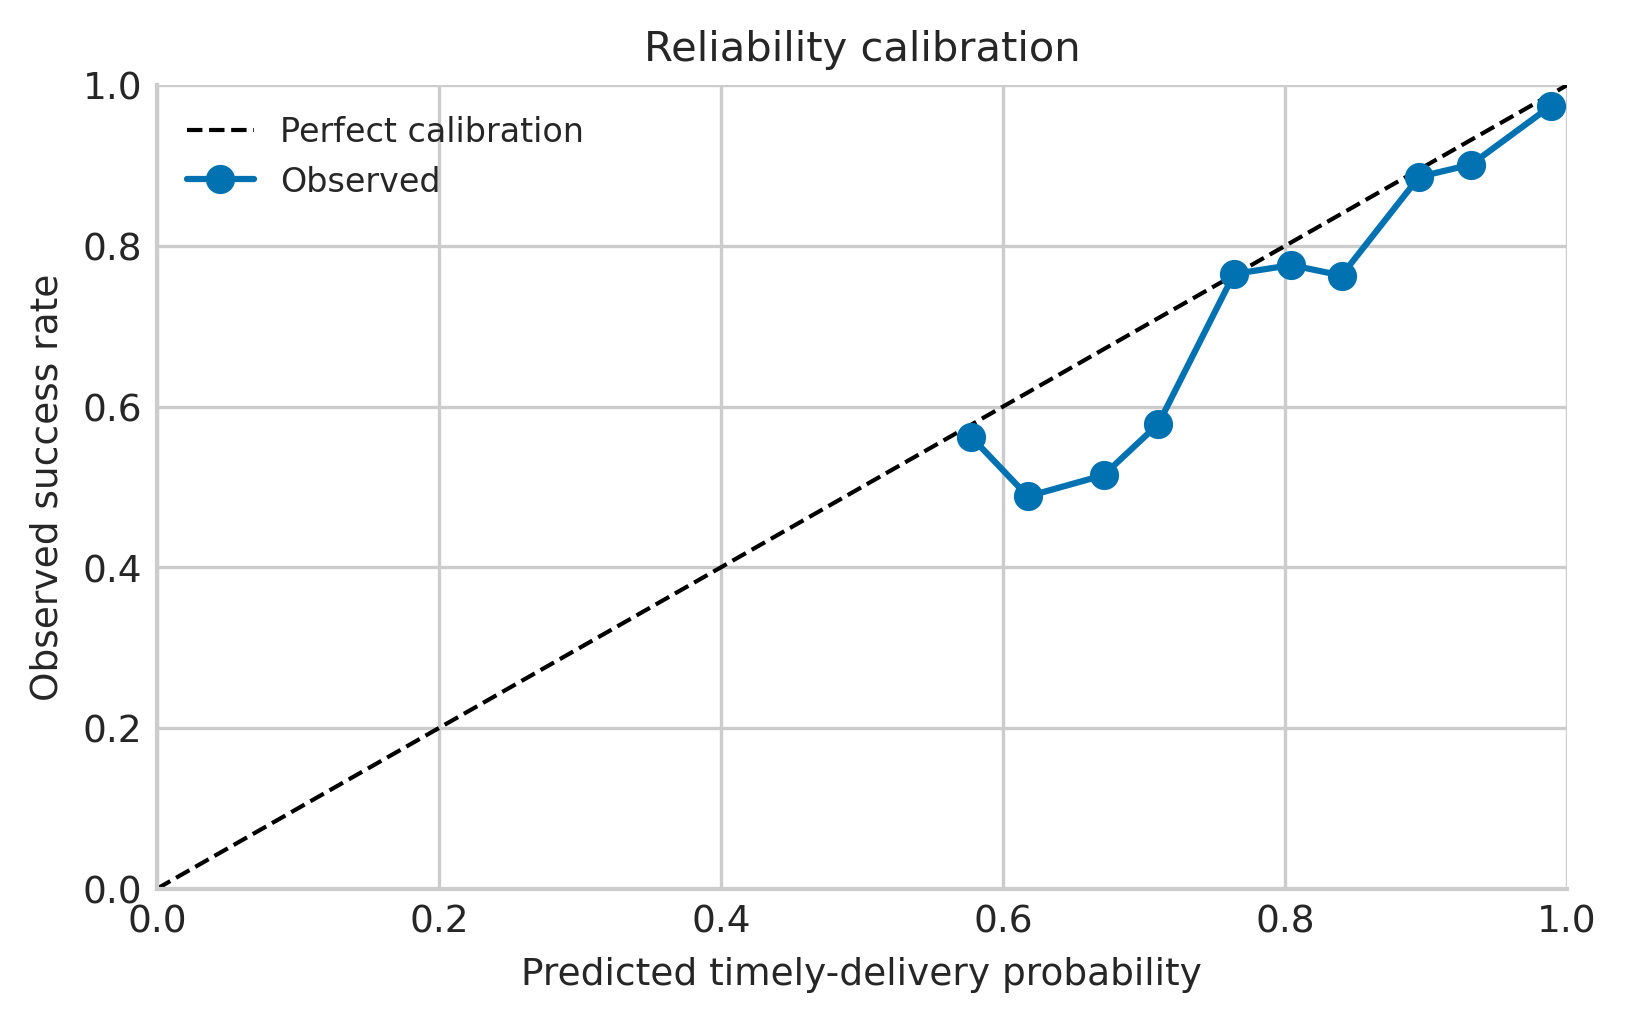
\includegraphics[width=\textwidth]{reliability_calibration.png}
\\[-2pt]\textbf{(b)} Reliability calibration
\end{minipage}
\caption{Additional diagnostics. Left: modeled utility, final exposure budget, and successful-update throughput. Right: calibration of predicted timely-delivery probability against observed success.}
\label{fig:completed_diagnostics}
\end{figure}

As a directional budget diagnostic, reducing the initial budget from 20 to 8 yielded GCDP objective $4.5213$ and final accuracy $0.5172$ in a single seed, whereas increasing it to 40 yielded objective $4.5255$ and accuracy $0.5315$. These one-seed values motivate a multi-seed budget sweep but are not used for significance claims.

% Keep all experimental tables and figures within the Evaluation section.
\FloatBarrier

\section{Discussion}

Protection strength and delivery feasibility are coupled in deadline-constrained FL. A policy that reduces a threat-specific exposure measure may also increase processing, communication, or synchronization time, causing the protected update to arrive too late to affect the model. MP-RBPS makes this coupling explicit, but the resulting decision remains conditional on the quality of its inputs. In particular, $P_{\mathrm{rel},i}^t(q)$ must be calibrated, $R_{\mathrm{exp}}(q)$ must be tied to a stated threat and measurement procedure, and policy overhead must reflect the target hardware and SecAgg group size.

Admission based on link reliability can systematically favor stable terrestrial clients. The contribution and fairness terms provide control variables for this effect, but they do not prove fairness. Domain participation and data-coverage disparity must therefore be reported explicitly. Similarly, the exposure budget is an application-level scheduling state; it is neither a differential-privacy accountant nor a cryptographic security parameter.

The current model has three further limitations. First, EWMA supplies a historical prior rather than a trajectory forecast; location- or orbit-aware prediction requires time-correlated mobility traces. Second, the SecAgg model captures group-size-dependent overhead but abstracts protocol rounds and the identities of clients that drop out during recovery. Third, GCDP is optimal for each estimated per-round problem, not for the finite-horizon stochastic control problem induced by future budget and mobility states. These limitations motivate the calibration, trace-driven, exactness, and scalability studies in Section~\ref{sec:evaluation_protocol}.

\section{Conclusion}

This paper formulated deadline-constrained protected FL as a joint client--policy selection problem. MP-RBPS combines a mobility-informed reliability prior, expected on-time learning contribution, resource feasibility, group-size-dependent SecAgg feasibility, and a finite-horizon exposure budget. GCDP compresses each client's feasible actions and solves the resulting group-cardinality problem exactly for every round.

The completed study supports a narrow, testable claim: conditional on the estimated utilities and common traces, GCDP solves each round's group-cardinality assignment exactly. In the main CIFAR-10 experiment it achieves the largest modeled utility among the evaluated policies and reduces communication relative to the reactive and compression-only baselines, at the cost of scheduler computation. The controlled stress study shows a consistent objective advantage over fixed protection, while the sequential two-stage, greedy, and reactive policies remain competitive at other Pareto points. Joint decision-making is therefore useful when protection, deadline feasibility, and exposure budget are simultaneously active, but it is not uniformly dominant on every metric or operating regime. The accuracy results should not be conflated with universal learning superiority, and the exposure score is an application-level scheduling proxy rather than formal privacy. Threat-specific leakage calibration, device-level overhead measurements, and horizon-aware stochastic control remain important extensions.

\fontsize{8.5pt}{10pt}\selectfont
\section*{Acknowledgements}
The authors thank the members of the Information Engineering University research group for discussions and assistance with the experimental implementation.

\section*{Competing interests}
The authors declare that they have no competing interests or financial conflicts to disclose.

\section*{Funding}
This research did not receive any specific grant from funding agencies in the public, commercial, or not-for-profit sectors.

\section*{CRediT authorship contribution statement}
Wenyu Ma: Methodology, Software, Validation, Writing -- original draft. Tao Hu: Conceptualization, Formal analysis, Supervision, Writing -- review and editing. Xinlei Liu: Data curation, Investigation, Visualization, Validation. All authors approved the submitted version and accept responsibility for the work.

\section*{Data availability}
The code, configuration files, and anonymized experiment outputs supporting the findings are included in the accompanying reproducibility materials; a permanent repository DOI will be supplied at submission. No personally identifiable or human-subject data were used.

\section*{Declaration of generative AI and AI-assisted technologies in the manuscript preparation process}
During the preparation of this work, the authors used AI-assisted tools for language editing and formatting support. The authors reviewed and edited all generated material and take full responsibility for the content of the published article.

\bibliographystyle{elsarticle-num}
\bibliography{references}

\end{document}
